% !TeX program = lualatex
\documentclass[a5paper]{article}
\usepackage[body={10cm,17cm}]{geometry}
\usepackage[a5,center,off]{crop}

\usepackage{blindtext}
\usepackage{tikz}
\usetikzlibrary{calc}
\usepackage[utf8]{inputenc}
\usepackage{multicol}
\usepackage{pdflscape}
\usepackage{longtable}
\usepackage{xcolor}
\setlength{\columnsep}{2cm}
\usepackage{fancyhdr}
\usepackage{everypage}
\usepackage{lipsum}
\usepackage{array}
\usepackage{lipsum}
\usepackage{tikz}
\usetikzlibrary{fit,shapes.geometric}
\usepackage{setspace}
\usepackage{adjustbox}
\usepackage{fontspec}
\usepackage{titlesec}
\usepackage{titling}
\usepackage{rotating}
\usepackage{pdfpages}
\usepackage{xargs}                      % Use more than one optional parameter in a new commands

\newfontfamily\headingfont[]{parisienne}
\titleformat*{\section}{\Huge\headingfont}
\titleformat*{\subsection}{\LARGE\headingfont}
\titleformat*{\subsubsection}{\large\headingfont}

\usepackage[colorinlistoftodos,prependcaption,textsize=tiny]{todonotes}
\newcommandx{\unsure}[2][1=]{\todo[linecolor=red,backgroundcolor=red!25,bordercolor=red,#1]{#2}}
\newcommandx{\change}[2][1=]{\todo[linecolor=blue,backgroundcolor=blue!25,bordercolor=blue,#1]{#2}}
\newcommandx{\info}[2][1=]{\todo[linecolor=OliveGreen,backgroundcolor=OliveGreen!25,bordercolor=OliveGreen,#1]{#2}}
\newcommandx{\improvement}[2][1=]{\todo[linecolor=Plum,backgroundcolor=Plum!25,bordercolor=Plum,#1]{#2}}
\newcommandx{\thiswillnotshow}[2][1=]{\todo[disable,#1]{#2}}
\newcommand\YUGE{\fontsize{48}{60}\selectfont}

%\renewcommand{\thesection}{}
%\renewcommand{\thesubsection}{}
\setcounter{secnumdepth}{0}
\renewcommand{\contentsname}{Innehållsförteckning}

\newcommand*\circled[1]{\tikz[baseline=(char.base)]{
		\node[shape=circle,draw,inner sep=2pt, color=red] (char) {#1};}}

\newcounter{nodemarkers}
\newcommand\circletext[1]{%
	\tikz[overlay,remember picture] 
	\node (marker-\arabic{nodemarkers}-a) at (0,1.5ex) {};%
	#1%
	\tikz[overlay,remember picture]
	\node (marker-\arabic{nodemarkers}-b) at (0,0){};%
	\tikz[overlay,remember picture,inner sep=2pt]
	\node[draw,ellipse,color=red, thick,fit=(marker-\arabic{nodemarkers}-a.center) (marker-\arabic{nodemarkers}-b.center)] {};%
	\stepcounter{nodemarkers}%
}

\newcolumntype{N}{>{\raggedright\arraybackslash}p{3cm}}
\newcolumntype{L}{>{\raggedright\arraybackslash}p{8cm}}
\newcolumntype{Q}{>{\raggedright\arraybackslash}p{4cm}}
\newcolumntype{T}{>{\raggedright\arraybackslash}p{2.1cm}}

\newcommand{\defpage}{\newgeometry{left=1.2cm,bottom=1.2cm,top=1.2cm,right=1cm}}

\begin{document}
	
 \cleardoublepage
 
 	
\defpage
	
	
	\begin{titlepage}
		\pagestyle{empty}
		\newgeometry{top=1cm, left=2cm,bottom=0.1cm}
		\noindent
		\begin{tikzpicture}[remember picture,overlay, every node/.style={anchor=south west,inner sep=0pt}, x=1mm,y=1mm]   
		\node[opacity=1.0] (fig1) at (-3.3cm,-15cm)
		{\includegraphics[trim={12.5cm 17.2cm 0 0.0cm},clip, scale=1.35]{ornament.eps}};
		\end{tikzpicture}
		\par
		\noindent
		\fontspec{parisienne}
		\vspace*{2.0cm}
		\begin{center}
			\YUGE Emma och Johnnys bröllop
		\end{center}
		%\vfill
		\vspace*{7.5cm}
		\noindent
		{\huge \textsf{Nu jäklar ska det firas!}}
		\vskip\baselineskip
		\noindent
		\Large \textsf{6 Oktober 2018}
	\end{titlepage}
	\clearpage\mbox{}\clearpage
	\begin{titlepage}
	\fontspec{parisienne}
	\begin{center}
	\vspace*{2.2cm}
	\YUGE Välkomna
	\vspace*{1.2cm}	
	\end{center}
	\begin{center}
		\includegraphics[width=0.92\textwidth]{emmajohnny-bw.png}
	\end{center}
	\newpage
	\end{titlepage}
	
	
	%%%%%%%%%%%%%%%%%%%%%%%%%%%%%%%%%%%%
	% reset header and footer:
	\pagestyle{fancy}
	\normalfont
	\lhead{}\chead{}\rhead{}
	\cfoot{\vspace*{-2\baselineskip}\thepage}
	\renewcommand{\headrulewidth}{0pt}
	
	\tableofcontents
	\newpage
	
	\section{Meny}
	\subsection*{Snittar}
	\begin{spacing}{1.3}	
		Västerbottenssnitt med gräslökskräm och rödbetsskott \\
		Polenta med sötpotatis och bönor \\
		Hush puppies med ärtor och chilli
	\end{spacing}
	\vspace{-0.1cm}
	
	\subsection*{Huvudrätt}
	\begin{spacing}{1.3}
		Amerikansk ek- och hickoryrökig högrev \\  
		Cajunkryddad och sotat norsk fjordlax med aska och frön   \\
		Getost med betor, picklade steklökar samt getostdressing. \\
		Krispig sötpotatis med gräslöksdressing och granatäpple   \\
		Roman- och frisésallad, med rostade valnötter, caesardressing och vitlökskrutonger \\
		Rostade morötter saltbakad rotselleri och solrosfrön      \\
		Rökta tomater i nötter, honung och puffat vete \\
		Rostad blomkål med tryffeljord  \\
		Surdegsbröd \\
		Örtsmör
	\end{spacing}	
	
	\vspace{-0.1cm}
	\subsection*{Fördessert och avec}
	\begin{spacing}{1.3}
		Citronbavaroise med dillpulver och smetanasorbet \\ 
		Ardbeg Islay Single Malt Scotch Whisky \\ 
		Aultmore Speyside Single Malt Scotch Whisky \\
		Baileys
	\end{spacing}
	\vspace{-0.1cm}
	
	\subsection*{Tårta}
	\begin{spacing}{1.3}
		Chokladmousse fylld med körsbär- och vaniljpannacotta, dekorerad med chokladflarn, vaniljmaränger och jordgubbsmakroner
	\end{spacing}

	
	\newpage
	\section{Dryck}
	Fritt fram att dräpa dryck i baren!
		
	\subsection*{Öl}
	\vspace{-0.2cm}
	\begin{itemize}
		\item Carlsberg Brewmasters American Pale Ale
		\item Åbro Brygg Mästarens Pale Ale 
		\item Mariestads Export
		\item Carlsberg
	\end{itemize}

	\subsection*{Cider och alkoläsk}
	\vspace{-0.2cm}
	\begin{itemize}
		\item Somersby Pear Cider
		\item Somersby Elderflower Lime Cider
		\item Hartwall Cool Grape Long Drink
	\end{itemize}
	 
		
	\subsection*{Vin}
	\vspace{-0.2cm}
	\begin{itemize}
		\item Rött, Zensa Primitivo 
		\item Vitt, Foot Of Africa Reserve Chenin Blanc 
	\end{itemize}

	\subsection*{Sprit i baren}
	\vspace{-0.2cm}
	\begin{itemize}
		\item Beefeater London Dry Gin
		\item Bacardí Razz
		\item Havana Club 7 
		\item Islay Mist Blended
	\end{itemize}

	
	\subsection*{Alkoholfritt}
	\vspace{-0.2cm}
	\begin{itemize}
		\item ... 
		\item ... 
		\item ... 
		\item ...
	\end{itemize}
	
	
	\newpage

\section{Svar tipspromenad}
\begin{center}
	\renewcommand{\arraystretch}{1.4}	
	\begin{tabular}{| p{0.25cm} | Q | T | T | T | }
		\hline
		&	Fråga	&	1	&	X	&	2	\\ \hline
		1	&	När träffades Johnny och Emma första gången?	&	\circletext{\textbf{På en konsert med Winnerbäck}}	&	En studentfest hos Gabbi	&	På Roberts 30årsfest	\\ \hline
		2	&	Vart gick brudparets första gemensamma utlandsresa?	&	\circletext{\textbf{Rom}}	&	Köpenhamn	&	Amsterdam	\\ \hline
		3	&	Vems idé var det att springa marathon?	&	\circletext{\textbf{Emmas}}	&	Alexander Hansens	&	Johnnys	\\ \hline
		4	&	Hur många marathonlopp har brudparet sprungit sammanlagt?	&	4	&	\circletext{\textbf{5}}	&	7	\\ \hline
		5	&	Hur länge har brudparet bott ihop	&	3år	&	\circletext{\textbf{4år}}	&	5år	\\ \hline
		6	&	Emmas tjejgäng från Lund kallas för BP. Vad står egentligen BP för?	&	\circletext{\textbf{Blodpudding}}	&	Bara Pattar	&	Bastupinglorna	\\ \hline
		7	&	Vilken rätt lagade Johnny på första daten?	&	\circletext{\textbf{Tacopaj}}	&	Hamburgare	&	Våffelmackor	\\ \hline
		8	&	Johnny kan många programmeringsspråk, men vilket kan Emma?	&	Matlab	&	C++	&	\circletext{\textbf{Java}} 	\\ \hline
		9	&	Vem bodde Johnny inte med i Prag?	&	Joel	&	\circletext{\textbf{Carl-David}}	&	Amir	\\ \hline
		10	&	Vilken var Johnny och Emmas första bil?	&	Saab 9-3	&	Kia Soul	&	\circletext{\textbf{Volvo V40}}	\\ \hline
		11	&	Hur många brädspel, exklusive expansioner, har brudparet?	&	\circletext{\textbf{22}}	&	25	&	27	\\ \hline
		12	&	Hur många tältnätter har Emma och Johnny gjort ihop?	&	16	&	19	&	\circletext{\textbf{21}}	\\ \hline
		
	\end{tabular}
\end{center}
\newpage

	\restoregeometry % restores the geometry
	
	\addcontentsline{toc}{section}{Bordsplacering}
	\thispagestyle{empty}
	\begin{turn}{90}
	\begin{tikzpicture}[remember picture, overlay]
	
	\node[inner sep=0pt] (borsplacering) at (-8.6, -4.2) {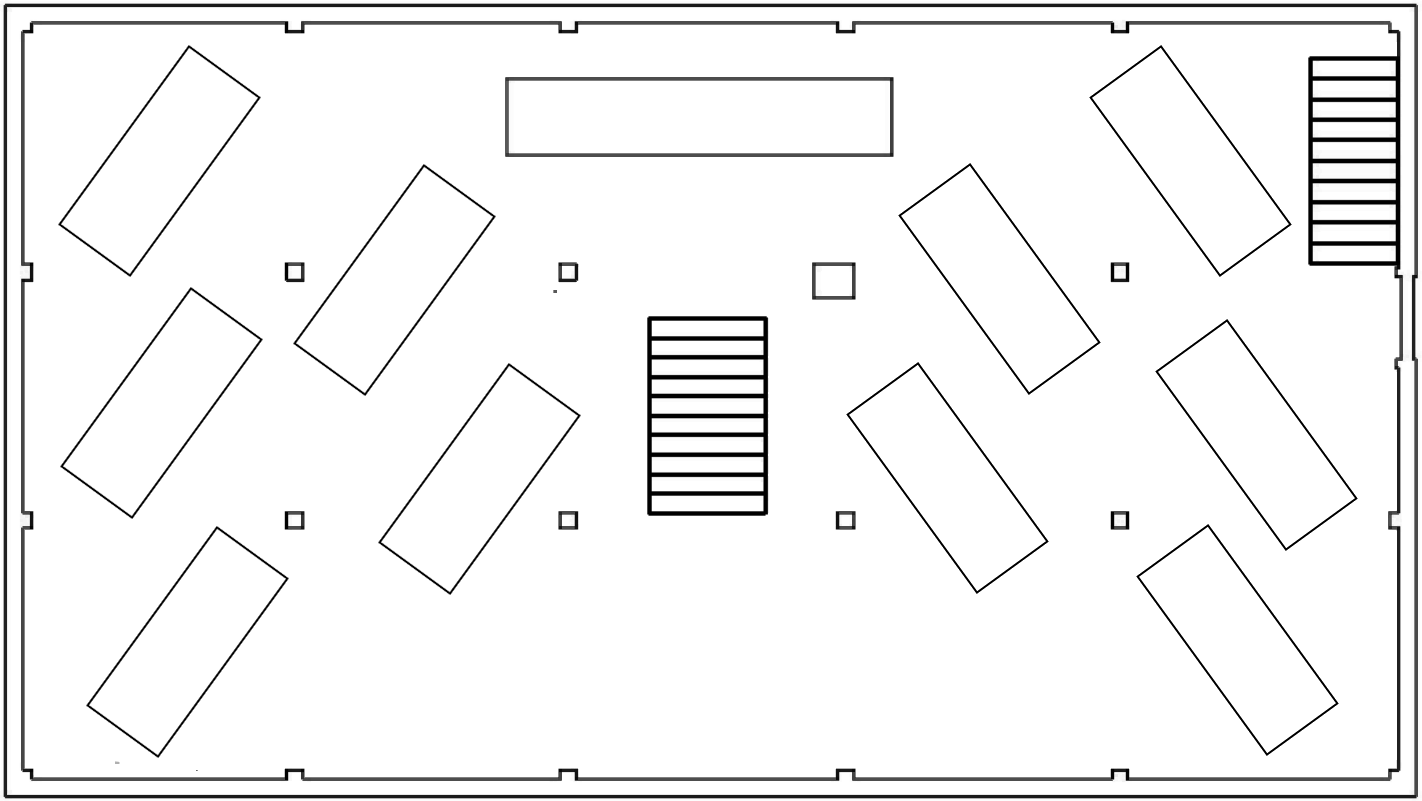
\includegraphics[width=1.4\paperwidth]{bordsplacering.png}} ;
	
	%\node[] (Bord 1) at (-16.5, -0.6) {\large \circled{1}};
	\node[rotate=54.5] (Bord 1) at (-16.5, -0.6) {\large Amsterdam};
	\node[] at (-8.8, 0) {\large Honnörsbordet};
	\node[rotate=54.5] (Bord 2) at (-16.5, -4.1) {\large Rom};
	% Rad 2		
	\node[rotate=54.5] (Bord 3) at (-16.4, -7.9) {\large Tjuonavagge};
	\node[rotate=54.5] (Bord 4) at (-13.3, -2.4) {\large Olserum};
	\node[rotate=54.5] (Bord 5) at (-12.0, -5.3) {\large Sommarhagen};
	\node[rotate=-54.5] (Bord 6) at (-4.5, -2.4) {\large Djurgårdsgatan};
	% Rad 3
	\node[rotate=-54.5] (Bord 7) at (-5.15, -5.4) {\large Skolgatan};
	\node[rotate=-54.5] (Bord 8) at (-1.8, -0.5) {\large Vätö};
	\node[rotate=-54.5] (Bord 9) at (-0.7, -4.6) {\large New York};
	\node[rotate=-54.5] (Bord 10) at (-0.8, -7.8) {\large Death Valley};
	
	\node[] (Page no) at (7.8,-11.5) {\thepage};
	\end{tikzpicture}
	\end{turn}
	
	
	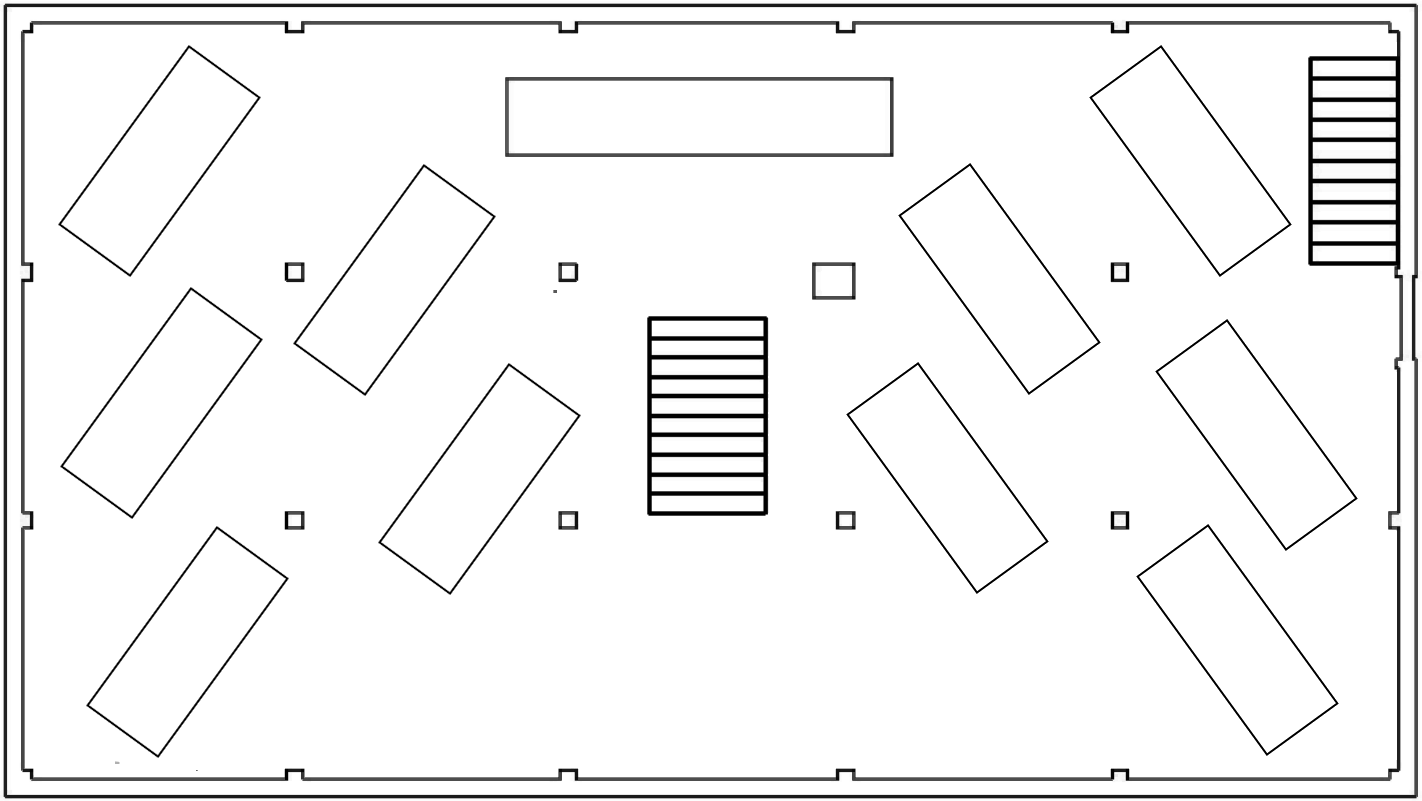
\includepdf[angle=90,pages=-,templatesize={105mm}{240mm},noautoscale=true,offset=-65 50]{bordsplacering.pdf}
	
	\restoregeometry
	\newpage
	
	%%
	
	\defpage
	\section{Gäster}
	
		\renewcommand*{\arraystretch}{1.8}
		\begin{longtable}[l]{N|L}
			%\caption{}\\
			%\hline
			\textbf{Namn} & \textbf{Beskrivning} \\ \hline
			\endfirsthead \hline
			%\endhead
			\multicolumn{2}{r}{\textit{Fortsättning på nästa sida}} \\ \endfoot
			\hline
			\endlastfoot
				Alexander Hansen	&	Sambo med brudens lillasyster. Biodlande stockholmsbo. Snabb som en iller i skogen, gärna jagandes kontroller och kantareller	\\
				Alexander Vidar	&	Vän från scouterna och balpartner till bruden. Kaffeälskande göteborgsbo 	\\
				Amir Mothagi	&	Vän till brudgummen från universitetet. Stockholmsbo som levde rövare med brudgummen i Prag. Sambo med Lara 	\\
				Andree Krantz Rosenquist	&	Vän till brudgummen från gymnasiet. Tranåsbo med nära band till USA	\\
				Anna Joelsson	&	Vän till bruden från universitetet och medlem i BP. Orkesterspelande lantmätare, ständigt på resande fot.	\\
				Anna Merkel Möller	&	Faster till brudgummen. Till vardags rektor i Eslöv, älskar skidåkning, vandring och resor   	\\
				Anna Möller	&	Vän till bruden från universitetet och medlem i BP'. Lantmätare i Uppsala, med rötter i Strängnäs som gärna sjunger i skalor. Sambo med Erik P.	\\
				Anna Våhlin	&	Vän till bruden från gymnasiet. Pysslig Linköpingsbo som gärna hänger på Gotland.	\\
				Anna-Ida Bergström	&	Fru till brudens kusin Mikael. Dalkulla boende i Stockholm. Skidtränare med stort löpintresse.	\\
				Annabel Merkel	&	Kusin till brudgummen. Hästintresserad med stort resintresse. Boendes i Malmö, roomie med magiska kaninen Merlin	\\
				Annika Andersson	&	Vän till bruden från universitetet och medlem i BP. Lantmätare från Eslöv, nu boende i Ängelholm. En hejare på att göra shots. Sambo med Björn A. \\
				Axel Merkel	&	Kusin till brudgummen och TM kvällen till ära. Bor och doktorerar i Molde, Norge. Föredetta roommate med brudgummen, på den tiden då broccoli var för dyrt 	\\
				Birgitta Merkel	&	Farmor till brudgummen. Bridgespelare, reser gärna både utrikes och inrikes till släkt och vänner. 	\\
				Björn Andersson	&	Sambo till Annika. Stor BP-supporter. Trodde vid tillfälle att bruden var frireligös.	\\
				Björn Karmbro	&	Morfar till brudgummen. Golfspelare med IT-intresse, går gärna promenader.  	\\
				Camille Andersson	&	Barndomsvän till bruden. Katrineholmsbo som gillar pyssel, matlagning och promenader.	\\
				Carl Wiklund	&	Barndomsvän till brudgummen. Malmöbo och en grym vollybollspelare. Har parkerat brudgummens cykel på ett tak. Sambo med Maria B.	\\
				Carl-David Ekblom	&	Vän till brudgummen från universitetet. Föredetta paintballproffs, skidtok och allmän prylnörd. Sambo med Ida.	\\
				Caroline Ingemansson &	Vän till bruden från universitetet och medlem i BP. Lantmätare som var brudens bättre(?) hälft när de bodde i München. Gift med Victor.	\\
				Daniel Svärd	&	Vän och kollega till brudgummen. Gillar klättring och frilutfsliv. Sprungit marathon och åkt vasalopp med brudgummen.  Sambo med Erika.	\\
				Elin Nilsson	&	Sambo med Peter. Arbetar som lärare i Linköping, är intruktör på Friskis och springer mycket.	\\
				Elisabet Ingmanson	&	Mormor till bruden. Hundälskare som numera är kattägare. Har köket tapetserat med teckningar från barnbarnen och dricker gärna kaffe.	\\
				Ellen Lynghed	&	Sambo med Hampus. Malmöbo med stort intresse för brädspel och sur egna barnkläder.	\\
				Emma Thorstenson	&	Vän till brudgummen från universitetet. Second hand- och vintageintresserad linköpingsbo. Sambo med Roger.	\\
				Erik Brattsröm	&	Vän till brudgummen från universitetet. Ägare till både bil, båt och motorcykel. OBS! Lägg honom ej i solen, han bränner sig lätt. Sambo till Matilda.	\\
				Erik Persson	&	Sambo med Anna M. Bandyspelande uppsalabo med rötter i Edsbyn. 	\\
				Erika Holmer	&	Sambo med Daniel. Friluftsintresserad klättrare som helst tar sig fram till fots.	\\
				Fia Storkull	&	Sambo med Jonathan.  Har sommarstuga med obligatorisk bastu i Finland. Bor i samma BRF som brudens föräldrar.	\\
				Fredrik Valdeson	& Sambo med Laura. Instrumentspelande Uppsalabo med intresse för runskrift.	\\
				Gabriella Hedin	&	Brudens storasyster. Älskar klättring och att vattna trädgårdslandet. Snabb i spåret men har inte än vågat sig på marathon. Sambo med Robert J.	\\
				Gunilla Hedin	    & Faster till bruden. Dalabo som gärna spenderar sommaren på Vätö och vintern på skidor.	\\
				Gustav Svanfeldt	& Vän och kollega till brudgummen. Har kört Iron man med brudgummen. Stort intresse för cyklar och ölbryggning.	\\
				Gustav Svebring	&	Gift med Malin S. Lantmätare och ett av BP:s största fan. Golfspelande malmöbo.	\\
				Hampus Lynghed	&	Vän till brudgummen från universitetet. MFF och brädspel står högt upp på Hampus prioritetslista 	\\
				Hanna Jonsson	&	Sambo med Henrik. Läkare som tältat med brudparet under Urkultfestivalen. Bor annars i Göteborg. 	\\
				Hedvig Hedin	&	Brudens kära mor. Golfspelare och nybliven husägare i välkänt område. Har givit bruden sitt mat och bakintresse.	\\
				Helena Niwong	&	Kusin till bruden. Från början dalkulla men numera bosatt i Stockholm. Vandrar och cyklar gärna med familjen.	\\
				Helena Sjöström	&	Vän till bruden från gymnasiet. Rest runt med bruden i Asien och flyttade tillsammans med  bruden till Lund.	\\
				Henrik Söderström	&	Vän till brudgummen från universitetet. Festerist ihop med brudgummen, byggde tillsammans en eldsprutande saucer. Sambo med Hanna.	\\
				Ida Grandell	&	Sambo med Carl-David. Tävlar med hunden Njállu. Rider och är gärna i stugan i Dalarna.	\\
				Jacob Lidman	&	Sambo med Maria K. Doktorand boende i Stockholm med ett stort ölintresse. 	\\
				Jeanette Bosund	&	Vän till bruden från universitetet och medlem i BP.  Hundälskande lantmätare bosatt i Lund. Gift med Karl B.	\\
				Joel Säll	&	Vän till brudgummen från universitetet. Kombo med brudgummen under utlandsstudier i Prag. Projekterar gärna runt huset i Knivsta. Sambo med Malin.	\\
				Jonas Merkel	&	Brudgummens far. Nyfunnet MTB-intresse och tvåfaldig svensk klassiker-medaljör.	\\
				Jonatan Hermansson	&	Vän till brudgummen från gymnasiet. Grillmästare som förespråkar mycket tändvätska och höga lågor. Till vardags pressekreterare i Riksdagen. Sambo med Fia.	\\
				Jörgen Möller	&	Gift med brudgummens faster Anna. Finurlig ingenjör med stort teknik och prylintresse. Har dragit brudgummens axel ur led.	\\
				Kalle Bosund	&	Sambo med Jeanette och BP-fantast. Tränar gärna, bor i Lund med hund och barn.	\\
				Katja Wigren	&	Barndomsvän till bruden. En hotta-brud som alltid hittar på tokigheter med bruden. Har bott i bland annat Italien, Kanada och nu Åre.	\\
				Kjell Pollack	&	Gift med brudens faster Gunilla. Näst efter flintastek går kottar varmt på grillen i stugan på Vätö.	\\
				Kristina Hedin	&	Brudens lillasyster. En fena på bin och avfall och har ännu inte slagit brudens tid på Göteborgsvarvet. Sambo med Alexander H.	\\
				Lara Borges	&	Sambo med Amir. Lärde känna brudgummen i Prag. Brudgummen har övernattat hemma hos Laras mor i Portugal.	\\
				Lars Johannesson	&	Sambo till brudgummens kusin Maja. Hemflyttad från Uppsala till Lund. Inte rädd för att kleta ner sig i Tjurruset.	\\
				Laura Betnér	&	Barndomsvän till bruden. Berest språkvetare som inte är rädd för att ta ton. Bryter fortfarande på småländska trots många år på schlätta och nu i Uppsala. Favoritfilm: Pearl Harbour. Sambo med Fredrik.	\\
				Lennart Hedin	&	Brudens far. En förkärlek till golf, kaffe och mjölkchoklad. Stammis på biblioteket och har gett bruden sitt läsintresse.	\\
				Linda Eriksen	&	Gift med Robert E. Boende utanför Mjölby och har stort hästintresse som äldsta dottern redan har ärft.	\\
				Louise Selga	&	Brudgummens kusin Stefans flickvän. Bakintresserad Lundabo som precis påbörjat en industridoktorandtjänst på SLU. 	\\
				Magnus Merkel	&	Brudgummens farbror. Kör elcykel och äter gärna god mat. Är i sommarstugan i Loftahammar så länge katten inte säger ifrån.	\\
				Maja Möller	&	Kusin till brudgummen. Djur- och naturälskare på både arbetet och fritiden. Matte till jaktlabradoren Aslan och nyligen hemflyttad till Skåne. Sambo med Lars.	\\
				Malin Lindström	&	Sambo med Joel. Bosatt i Knivsta men hänger gärna i sommarstugan utanför Motala. Jobbar på Uppsala universitet men är nu föräldaledig.	\\
				Malin Svebring	&	Vän till bruden från universitetet och medlem i BP. Lantmätare som jobbar med nya polishögskolan i Malmö. Bruden och Malin fann varandra med sin gemensamma scoutbakgrund. Gift med Gustav.	\\
				Maria Busck	&	Sambo med Carl. Influencer bosatt i Malmö med rötter i Hälsingland. 	\\
				Maria Karlsson	&	Barndomsvän med bruden och TM kvällen till ära. Stockholmsbo som gärna spenderar tid i sommarstugan utanför Söderköping. En orsak till att familjen Hedin hade två telefonnummer.	\\
				Marie Ericsson	&	Vän till bruden från universitetet och medlem i BP. Smålänning och lantmätare vars skratt smittar av sig. Äger stuga och skog men arealen kan vara svår att komma ihåg.	\\
				Marie-Louise Merkel	&	Mor till brudgummen. Ses ofta på långa hundpromenader eller på någon sina många cyklar.  	\\
				Matilda Arro	&	Sambo Erik B. Linköpingsbo som jobbar samtidigt som hon läser till läkare, resterande tid går till häst och hund. 	\\
				Mattias Kardell	&	Barndomsvän till brudgummen. Lärde känna brudgummen via SS Allians. Flyttat tillbaka till schlätten efter flera år i Göteborg.	\\
				Mikael Bergström	&	Kusin till bruden. Stockholmsbo men tidigare dalmas. Bygger på stugprojekt på sommaren och skjutsar till skidbackar på vintern. Gift med Anna-Ida.	\\
				Moa Chley Tegnelund	&	Vän till bruden från universitetet och medlem i BP. Lantmätare och stolt norrbottning boende i Malmö. Gillar beachvolleyboll och resor med rosabussarna.  	\\
				Ooy Ingmanson	&	Brudens morbror Pers fru. Trebarnsmor och en hejare på att klippa gräsmattan.	\\
				Per Ingmanson	&	Brudens morbror. Har släktens rekord på marathon. Skogsägare som gärna jagar. 	\\
				Per Wahlstedt	&	Sambo till brudgummens syster Rebecka. Stor frisbeenörd som då och då bulkar på gymmet. 	\\
				Peter Levin	&	Vän till brudparet. Lärde känna brudparet via Runacedemy. Driven idrottslärare som är snabb i löpspåret.	\\
				Rebecka Merkel	&	Brudgummens lillasyster. Frisbee-älskande Lundabo som blåser fram på rullskidor i snöfattiga Skåne. Vinner gärna över sin bror i brädspel. Sambo med Per. 	\\
				Renisa Kokoneshi	&	Sambo till Andree. Chicagotjej som numera bor i Tranås och studerar på Linköpings universitet.	\\
				Rickard Skogh	&	Sambo Emma T. Boende i Målbäck utanför Åtvidaberg. Leder i Domino. \\
				Robert Eriksen	&	Barndomsvän till brudgummen. Lärde känna brudgummen via SS Allians. Whiskyentusiast och har många gånger slagit brudgummen i TV-spel. Gift med Linda. 	\\
				Robert Janson	&	Emmas storasysters sambo och nära vän till brudgummen. Klätterapa och chiliodlare på vars 30-årsfest bruden och brudgummen träffades.	\\
				Roger Alne	&	Sambo med Sanna. Norsk brandingenjör boende utanför Oslo, renoverar hus och är tvåbarnsfar.	\\
				Roger Österback	&	Morbror till brudgummen. Linköpingsbo och snickare som gärna drar upp en gös eller två.	\\
				Sanna Lowén	&	Vän till bruden från gymnasiet, numera boende utanför Oslo. Favvodryck på gymnasiet efter sena kvällar var nyponsoppa. Sambo med Roger A.	\\
				Siv Karmbro	&	Mormor till brudgummen. Åker gärna på kryssningar med Björn och goda vänner.	\\
				Stefan Möller	&	Kusin till brudgummen. Nyexaminerad Uppsala-psykolog och återigen Lunda-bo. Reser gärna och har varit i de flesta världsdelar. Tillsammans med Louise.	\\
				Stefan Wass	&	Vän till brudgummen från gymnasiet och bestman kvällen till ära. Motorcykelförsäljare som sprungit in på 36:e plats på Göteborgsvarvet.	\\
				Thomas Niwong	&	Gift med brudens kusin Helena. Dalmas, numera stockholmsbo. Syns inte i rutan men verkar i bakgrunden.	\\
				Tobias Möller	&	Kusin till brudgummen. Boende i Lund, fotbollsspelare och stor MFF-supporter.	\\
				Victoria Wahlbom Hellström	&	Vän till brudparet. Ironmaniac med många cyklar som sprungit många långa ibland isiga löprundor med brudparet. Sambo med Gustav Svanfeldt.	\\
				Victor Ingemansson	&	Gift med Caroline och BP-stalker. Malmöbo men IFK Göteborgssupporter som besegrat Kullamannen dubbeldöden och sprungit marathon med brudparet.	\\
				Wiktor Holstenson	&	Vän till brudgummen från gymnasiet. Norrköpingsbo och sportfiskare med båten ständigt på släp. Friterar goda pommes till efterfesten. 	\\
		\end{longtable}
	
	\newpage
		
	\section{Sånger}
	
	\subsection{Sång 1 - Jag har aldrig var't på snusen}
		\textit{Melodi: O, hur saligt att få vandra} \\
		
		\noindent 
		Jag har aldrig varit på snusen \\ 
		aldrig rökat en cigarr, halleluja \\ 
		Mina dygder äro tusen \\ 
		inga syndiga laster jag har \\ 
		Jag har aldrig sett nåt naket \\ 
		inte ens ett nyfött barn, halleluja \\ 
		Mina blickar går mot taket \\ 
		därmed undgår jag frestarens garn \\ 
		
		\noindent
		Halleluja, Halleluja… \\ 
		
		\noindent
		Baccus spelar på gitarren \\ 
		Satan spelar på sitt handklaver \\ 
		alla djävlar dansar tango \\ 
		säg, vad kan man väl önska sig mer? \\ 	
		
		\noindent
		Jo att alla bäckar vore brännvin \\
		Stångån full av bayerskt öl \\
		konjak i varenda rännsten \\
		och punch i varendaste pöl, \\
	
		\noindent
		Halleluja, Halleluja…
	\newpage
	\subsection{Sång 2 - Bordeaux, Bordeaux}
		\textit{Melodi: I sommarens soliga dagar} \\
		
		\noindent
		Jag minns än idag hur min fader \\
		kom hem ifrån staden så glader \\
		och rada’ upp flaskor i rader \\
		och sade nöjd som så: \\
		”Bordeaux, Bordeaux!” \\
		
		\noindent 
		Han drack ett glas, kom i extas, \\
		och sedan blev det stort kalas. \\
		Och vi små glin, ja vi drack vin \\
		som första klassens fyllesvin. \\
		Och vi dansade runt där på golvet \\
		och skrek så vi blev blå:\\
		”Bordeaux, Bordeaux!” \\

	\subsection{Sång 3 - Feta Fransyskor}
		\textit{Melodi: Marche Militaire} \\
		
		\noindent
		Feta fransyskor som svettas om fötterna, \\
		de trampar druvor som sedan ska jäsas till vin. \\
		Transpirationen viktig é, ty den ge’ fin bouquet. \\
		Vårtor och svampar följer me’ men vad gör väl de’? \\
		
		\noindent
		För… vi vill ha vin, vill ha vin, vill ha mera vin, \\
		även om följderna blir att vi få lida pin. \\
		Flaskan och glaset gått i sin. \\
		Hit med vin, mera vin! \\
		Tror ni att vi är fyllesvin? \\
		JA! (fast större) \\
				
		\newpage
		
		
\subsection{Sång 4 - Lantmätarens testamente}
\textit{Mellodi: She'll be coming down the mountin} \\

\noindent

\noindent
:,: Du ska få mitt lod med snöre när jag dör :,: \\
ty i paradisets hagar \\
gälla inte Newtons lagar.\\
Du ska få mitt lod med snöre när jag dör. \\

\noindent
:,: Du ska få mitt gamla mätband när jag dör :,: \\
ty där uppe uti etern \\
får det slå på kilometern \\
Du ska få mitt gamla mätband när jag dör. \\

\noindent
:,: Du ska få min gamla lagbok när jag dör :,: \\
ty i kalla, blöta kalken \\
gäller inte jordabalken \\
Du ska få min gamla lagbok när jag dör. \\

\subsection{Sång 5 - Siffervisan}
\textit{Melodi: Ritsch, ratsch} \\
	
\noindent
1, 2, 75, 6, 7, 75, 6, 7, 75, 6, 7 \\
1, 2, 75, 6, 7, 75, 6, 7, 73 \\
107, 103, 102 \\
107, 6, 19, 27 \\
17, 18, 16, 15 \\
13, 19, 14, 17 \\
19, 16, 15, 11 \\
8, 47! \\

\newpage

\subsection{Sång 6 - Finland}
\textit{Melodi: Högt över havet} \\

\noindent 
Finland är Finland och Finland är bra. \\
Dom har en pipeline med sprit från Moskva. \\
Bada Bastu, piska med ris, \\
hacka hål i is. \\

\noindent 
Danmark är Danmark och Danmark är bra. \\
Dom har en jungfru som sitter så bar. \\
Röde pölsor med Tuborg och lök, \\
vi köpte billig krök \\

\noindent 
Norge är Norge och Norge är bra. \\
Dom har den olja som vi vill ha. \\
Dyrt i baren ett jävla pris, \\
klubba säl med is. \\

\noindent 
Island är Island och Island är bra. \\
Kriser, vulkaner och hästar dom har. \\
Jag fiser i geisern vad var det jag sa, valspeck varje dag. \\

\noindent 
Sverige är Sverige och Sverige är bäst. \\
Ingvar Kamprad han tjänar mest. \\
Ullared, Abba och Absolut, \\
Nu är visan slut. \\


\subsection{Sång 7 - Mera brännvin i glasen}
\textit{Melodi: Internationalen} \\

\noindent
Mera brännvin i glasen, \\
mera glas på vårt bord, \\
mera bord på kalasen, \\
mera kalas på vår jord. \\
 
\noindent
Mera jordar kring månen, \\
mera månar kring Mars, \\
mera marscher till Skåne, \\
mera Skåne, Gud bevars, bevars, bevars! \\


\newpage
\subsection{Sång 8 - Spritbolaget}

\textit{Melodi: Du käre lille snickerbo’} \\

\noindent
Till spritbolaget ränner jag \\
och bankar på dess port. \\
Jag vill ha nå’t som bränner bra \\
och gör mig sketfull fort. \\
Expediten sade: ”Godda’, \\
hur gammal kan min herre va’? \\
Har du nå’t leg, ditt fula drägg? \\
Kom hit igen när du fått skägg!” \\

\noindent
Nej, detta var ju inte bra, \\
jag ska bli full ikväll. \\
Då plötsligt en idé fick jag: \\
De har ju sprit på Shell! \\
Många flaskor stod där på rad, \\
så nu kan jag bli full och glad. \\
Den röda drycken åkte ner… \\
Nu kan jag inte se nå’t mer	\\
	
\subsection{Sång 9 - Strejk på pripps}
\textit{Melodi: I natt jag drömde}\\

\noindent
I natt jag drömde något som,\\
jag aldrig drömt förut.\\ 
Jag drömde det var strejk på Pripps\\
och alla ölen var slut.\\
Jag drömde om en jättesal\\
där ölen stod på rad.\\
Jag drack så där ett tjugotal\\
och reste mig och sa;\\

\noindent
Armen i vinkel\\
blicken i skyn\\
så var det menat\\
whisky och renat\\
vårt mål alkohol!\\
För dem som tål! - SKÅL\\
\newpage


\section{Tack}
Stort tack till alla er som är här och hjälper oss att förgylla vår dag! \\ \\
Ett extra stort tack till toastmasters, bestman och tärna för era fantastiska insatser!






\end{document}